\newpage
\section{Scanning probe microscopy editor}
When simulating a 3D structure such as a large area contact one often wants to map the resistance between an x,z point on the surface of the device and the charge extraction contact. This tool is used to apply voltages systematically over z,x regions to map out voltage or resistance profiles in space.  This tool is usually used with either full 2/3D drift diffusion simulations or the 3D large area electrical circuit model. There is more about this tool in Section \ref{ref:la}.

\begin{figure}[H]
\centering
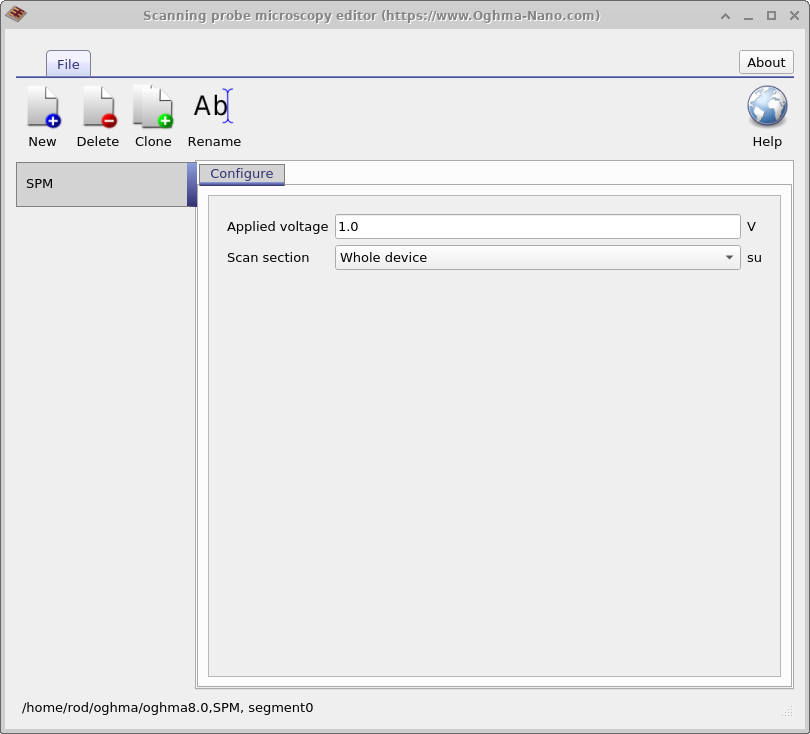
\includegraphics[width=0.7\textwidth,height=0.5\textwidth]{./images/sim_editors/spm.png}
\caption{The scanning probe microscopy editor}
\label{fig:spm_editor}
\end{figure}
